\documentclass[12pt, twoside]{article}
\usepackage[letterpaper, margin=1in, headsep=0.5in]{geometry}
\usepackage[english]{babel}
\usepackage[utf8]{inputenc}
\usepackage{amsmath}
\usepackage{amsfonts}
\usepackage{amssymb}
\usepackage{tikz}
%\usetikzlibrary{quotes, angles}

\usepackage{graphicx}
\usepackage{enumitem}
\usepackage{multicol}

\usepackage{fancyhdr}
\pagestyle{fancy}
\fancyhf{}
\renewcommand{\headrulewidth}{0pt} % disable the underline of the header

\fancyhead[RE]{\thepage}
\fancyhead[RO]{\thepage \\ Name: \hspace{3cm}}
\fancyhead[L]{BECA / Dr. Huson / 10th Grade Geometry\\* Unit 9: Angle Relationships\\28 March 2019}

\begin{document}
\subsubsection*{9-3 Do Now: Triangle external angles}
  \begin{enumerate}

      \item Given $m\angle R=47^\circ$ and $m\angle UST=103^\circ$. Find $m\angle U$.\\[1cm]
        \begin{tikzpicture}
          %\draw [->, thick] (0,0)--(5,5);
          \draw [<-, thick] (8,0)--(0,0)--(3,3)--(4.5,0);
          \draw [fill] (0,0) circle [radius=0.05] node[below]{$R$};
          \draw [fill] (4.5,0) circle [radius=0.05] node[below]{$S$};
          \draw [fill] (3,3) circle [radius=0.05] node[right]{$U$};
          \draw [fill] (7,0) circle [radius=0.05] node[below]{$T$};
        \end{tikzpicture}
        \vspace{3cm}

      \item In  $\triangle ABC$ shown below, side $\overline{AC}$ is extended to point $D$ with $m\angle DAB=(180-2x)^\circ$, $m\angle C=(x-10)^\circ$, and $m\angle B=(3x+10)^\circ$.
        \begin{center}
          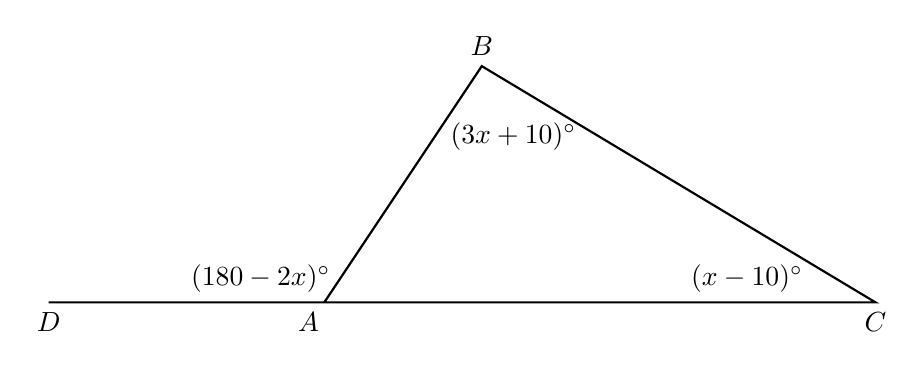
\begin{tikzpicture}
            \draw [thick](-1.5,0)node[below]{$D$}--
              (1.8,0)node[below]{$A$}--
              (9,0)node[below]{$C$}--
              (4,3)node[above]{$B$} --(2,0);
              \node at (2.2,0)[above left]{$(180-2x)^\circ$};
              \node at (8.2,0)[above left]{$(x-10)^\circ$};
              \node at (4.4,2.4)[below]{$(3x+10)^\circ$};
          \end{tikzpicture}
        \end{center}
        What is $m\angle BAC$?

\newpage
  \item Given $P(3,0)$ and $Q(9,-2)$, find the length of $\overline{PQ}$. Leave  the result as a simplified radical.
      \vspace{4cm}

  \item Triangle $\triangle TEN$ is graphed on the set of axes below. The vertices of $\triangle TEN$ have the coordinates $T(-1,-2)$, $E(8,1)$, and $N(3,6)$.
    \begin{center} %4 quadrant regents grid
    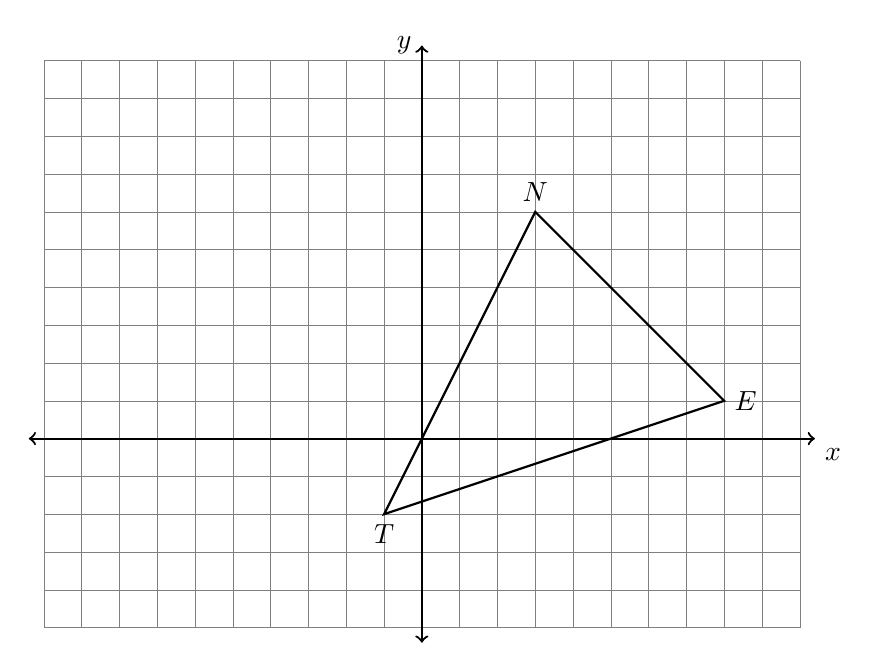
\begin{tikzpicture}[scale=.48]
      \draw [help lines] (-10,-5) grid (10,10);
      \draw [thick, <->] (-10.4,0) -- (10.4,0) node [below right] {$x$};
      \draw [thick, <->] (0,-5.4)--(0,10.4) node [left] {$y$};
      \draw [thick] (-1,-2) node[below] {$T$}--
      (8,1) node[right] {$E$}--
      (3,6) node[above] {$N$}--
      cycle;
      %\draw [fill] (5,0) circle [radius=0.1] node[above left] {$P$};
    \end{tikzpicture}
    \end{center}
    \begin{enumerate}
      \item Find the slope of the line segment $\overline{TE}$. \vspace{2.5cm}
      \item What is the slope of a line perpendicular to $\overline{TE}$? \vspace{1.5cm}
      \item Write down the equation of a line through $N$ perpendicular to $\overline{TE}$. (use the point slope formula, $y-y_N=m_\perp (x-x_N)$).  \vspace{1.5cm}
    \end{enumerate}

\end{enumerate}
\newpage
\setcounter{page}{1}
\subsubsection*{9-3 Homework: Triangle external angles}
  \begin{enumerate}

  \item On the graph below, draw $\overline{AB}$, with $A(-1,5)$ and $B(7,0)$, labeling the end points. Determine and state the coordinates of the midpoint $M$ of $\overline{AB}$ and mark and label it on the graph.\\
    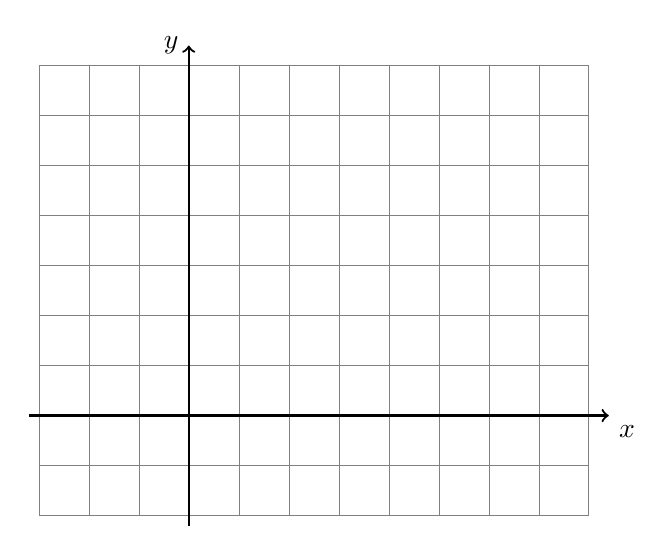
\begin{tikzpicture}[scale=.635]
      \draw [help lines] (-3,-2) grid (8,7);
      \draw [thick, ->] (-3.2,0) -- (8.4,0) node [below right] {$x$};
      \draw [thick, ->] (0,-2.2)--(0,7.4) node [left] {$y$};
    \end{tikzpicture}
    \vspace{1cm}

  \item In the diagram below, $\overleftrightarrow{AC}$ has endpoints with coordinates $A(-3,2)$ and $C(3, -7)$.
    \begin{center} %4 quadrant regents grid
      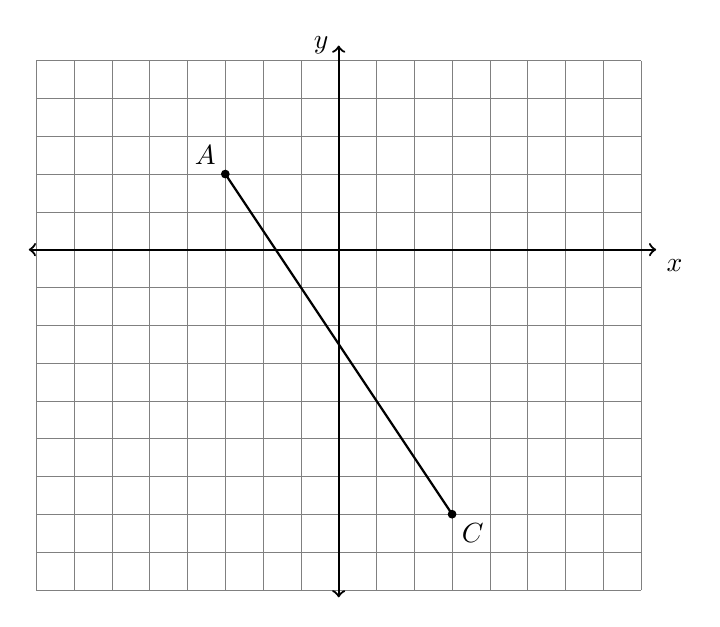
\begin{tikzpicture}[scale=.48]
        \draw [help lines] (-8,-9) grid (8,5);
        \draw [thick, <->] (-8.2,0) -- (8.4,0) node [below right] {$x$};
        \draw [thick, <->] (0,-9.2)--(0,5.4) node [left] {$y$};
        \draw [thick] (-3,2)--(3,-7);
        \draw [fill] (-3,2) circle [radius=0.1] node[above left] {$A$};
        \draw [fill] (3,-7) circle [radius=0.1] node[below right] {$C$};
      \end{tikzpicture}
    \end{center}
    If $B$ is a point on  and $AB {:} BC = 1{:}2$,  what  are  the  coordinates of $B$?

\newpage

  \item Given two parallel lines and a transversal, as shown. Apply the theorem, ``If a transversal intersects two parallel lines, then corresponding angles are congruent."
    \begin{center}
    \begin{tikzpicture}
      \draw [<->, thick] (1,2)--(9,2);
      \draw [<->, thick] (0,0)--(8,0);
      \draw [<->, thick] (4,-1)--(5.5,3);
      \node at (4.5,0.3) [left]{$5$};
      \node at (4.5,0.3) [right]{$6$};
      \node at (4.3,-0.3) [left]{$7$};
      \node at (4.3,-0.3) [right]{$8$};
      \node at (5.2,2) [above left]{$1$};
      \node at (5.2,2) [above right]{$2$};
      \node at (5,2) [below left]{$3$};
      \node at (5,2) [below right]{$4$};
    \end{tikzpicture}
    \end{center}
    \begin{enumerate}
      \item State the angle corresponding with $\angle 2$. \vspace{1cm}
      \item Given $m\angle 4 = 115^\circ$ and $m\angle 6 = 5x^\circ$. Find $x$. \vspace{3cm}
      \item Given $m\angle 7 = 65^\circ$. Find $m\angle 2$. \vspace{2cm}
      \item In a proof, what reason would justify $\angle 4 \cong \angle 5$? \rule{6cm}{0.15mm}
    \end{enumerate}

    \item The image of triangle $ABC$ after a translation is $\triangle A'B'C'$. Is the area of the triangle greater, smaller, or the same after the translation? Justify your answer.

\newpage

\item Express the result to the nearest thousandth.  %\vspace{0.5cm}
  \begin{multicols}{2}
    \begin{enumerate}
      \item $\cos 60^\circ = $ \vspace{0.5cm}
      \item $\tan 45^\circ =$
      \item $\sin 48^\circ = $ \vspace{0.5cm}
      \item $\cos 15^\circ =$
    \end{enumerate}
  \end{multicols}

  \item $\triangle ABC$ is shown with $m\angle C=90^\circ$. The lengths of the triangle's sides are $a$, $b$, and $c$.
    \begin{center}
      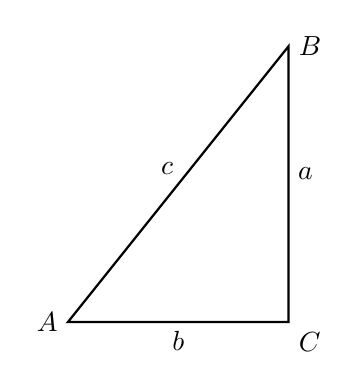
\begin{tikzpicture}[scale=0.7]
        \draw [thick]
        (0,0)node[left]{$A$}--
        (4,0)node[below right]{$C$}--
        (4,5)node[right]{$B$}--cycle;
        \node at (2,0)[below]{$b$};
        \node at (4,2.7)[right]{$a$};
        \node at (1.8,2.5)[above]{$c$};
      \end{tikzpicture} %\vspace{1cm}
    \end{center}
    Express each trigonometric ratio as a fraction of two variables.
    \begin{multicols}{2}
      \begin{enumerate}
      \item $\sin A =$ \vspace{0.5cm}
      \item $\cos A =$ \vspace{0.5cm}
      \item $\tan A =$
      \item $\sin B =$ \vspace{0.5cm}
      \item $\cos B =$ \vspace{0.5cm}
      \item $\tan B =$
    \end{enumerate}
  \end{multicols}

  \item Given right $\triangle JKL$ with $\overline{JK} \perp \overline{KL}$, $JL=11$, $m\angle J=29^\circ$.
    \begin{center}
      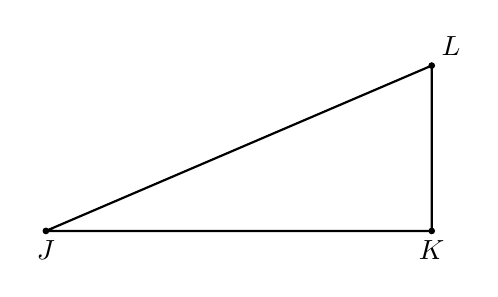
\begin{tikzpicture}[scale=0.7]
        \draw [thick](0,0)--(7,0)--(7,3)--(0,0);
        \draw [fill] (0,0) circle [radius=0.05] node[below]{$J$};
        \draw [fill] (7,0) circle [radius=0.05] node[below]{$K$};
        \draw [fill] (7,3) circle [radius=0.05] node[above right]{$L$};
      \end{tikzpicture}
    \end{center}
    \begin{enumerate}
      \item Find the length $JK$ \vspace{1.25cm}
      \item Find the length $KL$
    \end{enumerate}


\newpage

    \item Using  a  compass  and  straightedge,  construct  the  median  to  side $\overline{AC}$ in $\triangle ABC$ below.\\ (Leave all construction marks.)
      \vspace{1cm}
    \begin{center}
    \begin{tikzpicture}
      \draw [<->, thick]
        (0,0) node[left]{$A$}--
        (10,-2) node[right]{$B$}--
        (4,-5) node[below]{$C$}
        --cycle;
    \end{tikzpicture}
    \end{center}

      \vspace{2cm}

    \item With a compass and straightedge, construct a regular hexagon inscribed in a circle. (Leave all construction marks.)




  \end{enumerate}

  \end{document}






\newpage

  \item Given two vertical angles, $m \angle 1 = 5x+9$, $m \angle 2 = 6x-1$. Find $m \angle 1$.\\
  For full credit, check by comparing to $m\angle 2$.
      \begin{flushright}
      \begin{tikzpicture}[scale=.7]
        \draw [<->, thick] (0,-1.5)--(10,1.5);
        \draw [<->, thick] (2,3.5)--(7,-3.5);
        \node at (3,.4){1};
        \node at (6,-.6){2};
      \end{tikzpicture}
      \end{flushright}

  \item Given $\overrightarrow{BA} \perp \overrightarrow{BC}$, $m \angle ABD = 10x+15$, and $m \angle DBC = 5x$. Find $m \angle DBC$. \\[0.5cm]
  For full credit, show the check using both angle measures.
    \begin{flushleft}
    \begin{tikzpicture}[scale=1.3]
      \draw [<->, thick] (0,3)--(0,0)--(5,0);
      \draw [->, thick] (0,0)--(3.5, 2);
      \draw [-, thin] (0, 0.4)--(0.4, 0.4)--(0.4, 0);
      %\node at (3,.4){1};
      %\node at (6,-.6){2};
      \draw [fill] (0,0) circle [radius=0.05] node[below]{$B$};
      \draw [fill] (0,2) circle [radius=0.05] node[left]{$A$};
      \draw [fill] (4,0) circle [radius=0.05] node[below]{$C$};
      \draw [fill] (2.625, 1.5) circle [radius=0.05] node[below]{$D$};
    \end{tikzpicture}
    \end{flushleft}
    \vspace{3cm}

    \item Given the circle $C$ with circumference $12\pi$.
  \begin{enumerate}
    \item Write down the formula for the circumference of a circle and solve for the radius yielding a circumference of $12\pi$. \vspace{1cm}
    \item Find the area of the circle.
  \end{enumerate}
  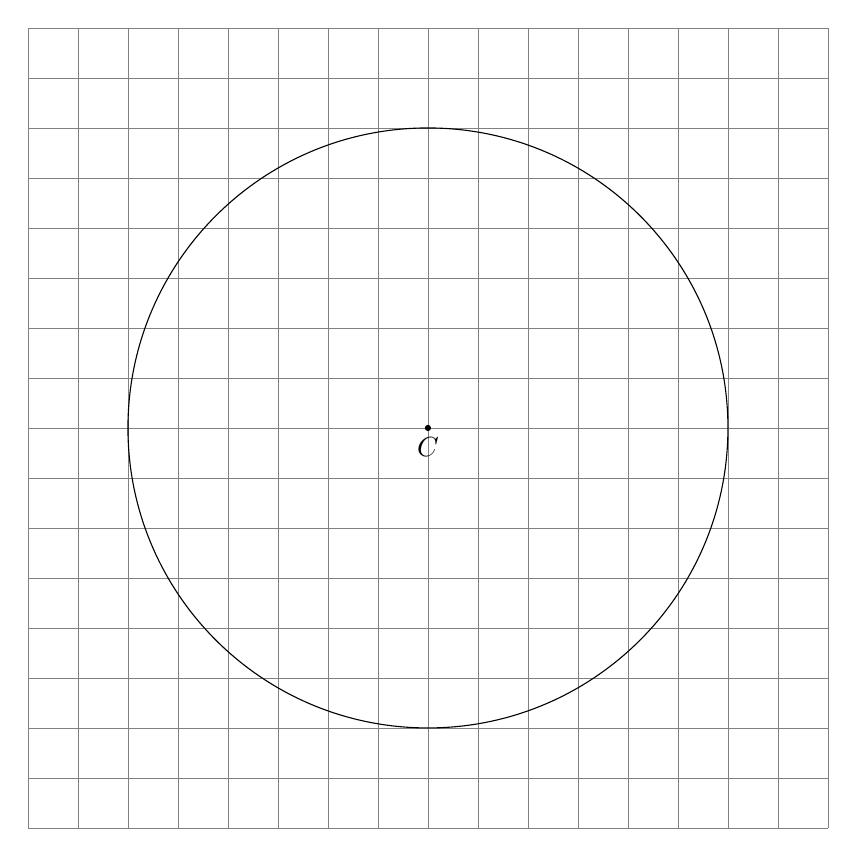
\begin{tikzpicture}[scale=.635]
    \draw [help lines] (-8,-8) grid (8,8);
    %\draw [thick, ->] (-2.2,0) -- (10.4,0) node [below right] {$x$};
    %\draw [thick, ->] (0,-2.2)--(0,10.4) node [left] {$y$};
    \draw (0,0) circle [radius=6] node[below]{$C$};
    \draw [fill] (0,0) circle [radius=0.05];
  \end{tikzpicture}

  \item On the graph, draw polygon ABCDEF with vertices A(1, 1), B(1, 4), C(3, 4), D(3, 7), E(8, 7), and F(8, 1). Find the perimeter and the area of the polygon.\\[1cm]
  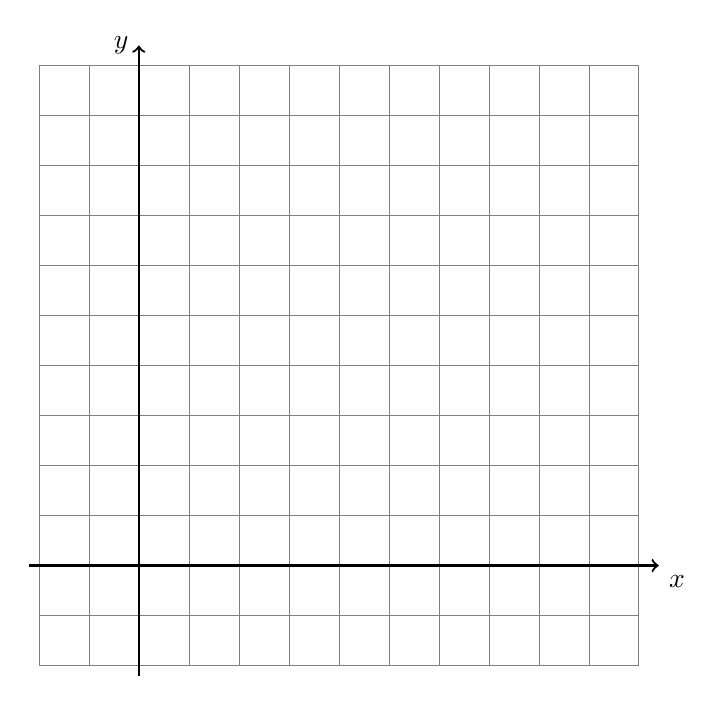
\begin{tikzpicture}[scale=.635]
    \draw [help lines] (-2,-2) grid (10,10);
    \draw [thick, ->] (-2.2,0) -- (10.4,0) node [below right] {$x$};
    \draw [thick, ->] (0,-2.2)--(0,10.4) node [left] {$y$};
  \end{tikzpicture}
  \vspace{2cm}

  \item Given a circle $O$ with radius $5$.
  \begin{enumerate}
    \item Find the circumference of $O$. \vspace{2cm}
    \item Find the area of $O$. \vspace{2cm}
  \end{enumerate}


\newpage

  \item Given $\overline{JKL}$, $JL=24$, and the point $K$ partitions $\overline{JL}$ in a ratio of 1:3.\\[0.5cm] Find ${JK}$. \\[1.5cm]
      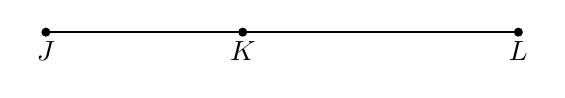
\begin{tikzpicture}
        \draw [-, thick] (1,0)--(7,0);
        \draw [fill] (1,0) circle [radius=0.05] node[below]{$J$};
        \draw [fill] (3.5,0) circle [radius=0.05] node[below]{$K$};
        \draw [fill] (7,0) circle [radius=0.05] node[below]{$L$};
      \end{tikzpicture} \vspace{3cm}
